\subsection{Bibliothèques utilisées (SFML)}\label{subsec:sfml}
SFML (\textit{Simple and Fast Multimedia Library}) est une bibliothèque C++ qui permet de créer des applications multimédia.
Elle est particulièrement adaptée pour le développement de jeux vidéo et d'applications graphiques.
Elle fournit des fonctionnalités pour la gestion des fenêtres, le rendu graphique, la gestion des événements, le son et la communication réseau.
En interne, elle s'appuie sur OpenGL, une API bas niveau, ce qui permet d'obtenir d'excellentes performances graphiques tout en restant simple d'utilisation.

SFML a été choisie pour plusieurs raisons :
\begin{itemize}
    \item \textbf{Simplicité d'utilisation} : Elle permet de se concentrer sur la logique applicative plutôt que sur des détails techniques complexes.
    \item \textbf{Documentation et communauté} : Sa documentation\cite{documentationSFML} est complète et une large communauté offre de nombreux exemples et ressources.
    \item \textbf{Multiplateforme} : La compatibilité avec Windows, Linux et macOS permet de développer l'application sans penser à la portabilité.
\end{itemize}

\subsection{Architecture de l'interface graphique}\label{subsec:architecture-de-l-interface-graphique}
\subsubsection{Organisation modulaire du code}\label{subsubsec:organisation-modulaire-du-code}
Pour garantir la lisibilité et la maintenabilité du code, l'interface graphique a été conçue de manière modulaire.
Chaque fonctionnalité est encapsulée dans une classe dédiée, permettant ainsi une séparation claire des responsabilités.
Par exemple, la gestion du véhicule, du circuit, des indicateurs de débogage sont traitées dans des modules distincts.
Cette approche facilite également l'ajout de nouvelles fonctionnalités sans modifier la structure existante.

\subsubsection{Présentation des classes principales}\label{subsubsec:presentation-des-classes-principales}
Plusieurs classes clés interagissent pour offrir une interface graphique cohérente et fluide.

\paragraph[Game]{La Classe \textbf{Game}}
C'est la classe principale du projet, elle orchestre l'application.
Elle initialise la fenêtre SFML, configure les vues (Game View et HUD View), gère le cycle de vie de la simulation (mise à jour, gestion des événements et rendu) et coordonne les interactions entre les différents modules.

Elle contient 3 fonctions principales :
\begin{lstlisting}[style=CStyle, label={lst:game_class}]
    void update();
    void render() const;
    void manageEvents();
\end{lstlisting}
Chaque fonction est appeller une fois par itération de la boucle principale de l'application et donc par image générer.
Voici leurs rôles respectifs :
\begin{itemize}
    \item \texttt{update()}, met à jour l'état de l'application en fonction du temps écoulé et des événements utilisateurs.
    \item \texttt{render()}, effectue le rendu graphique de la scène actuelle.
    \item \texttt{manageEvents()}, gère les événements à l'intérieur de l'application (clavier, souris), elle est appellé dans la fonction \texttt{update()}.
\end{itemize}

\paragraph[Circuit]{La Classe \textbf{Circuit}}
Elle représente, comme son nom l'indique, un circuit de conduite.
Elle est composé de différents segments de routes (comme une petite ligne droite, un petit virage, un grand virage, \dots).
Chaque segment est une portion de route qui peut être droite ou courbe, et la classe gère la connexion entre ces segments pour former une impression de circuit continue au niveau de l'affichage graphique. \\
Son fonctionnement interne permet, de l'extérieur de la classe, de simplifier la création de la route.
Il suffit de rajouter des segments de route dans le circuit en précisant l'angle à donner à la texture et s'il faut lui appliquer un effet mirroir, et la classe se charge de les relier entre eux.

L'extrait de code suivant permet de réaliser ce bout de circuit (fig.~\ref{fig:example_circuit_1}) :
\begin{lstlisting}[style=CStyle, label={lst:code_circuit}]
Circuit circuit;
circuit.setOrigin(ResourceType::Value::SEGMENT_SMALL_STRAIGHT);
circuit.join(ResourceType::Value::SEGMENT_S_TURN);
circuit.join(ResourceType::Value::SEGMENT_MEDIUM_TURN);
circuit.join(ResourceType::Value::SEGMENT_LARGE_TURN, 90);
circuit.join(ResourceType::Value::SEGMENT_U_TURN, 180);
circuit.join(ResourceType::Value::SEGMENT_U_TURN, 0, false, true);
circuit.join(ResourceType::Value::SEGMENT_LONG_STRAIGHT, 180);
\end{lstlisting}

\begin{figure}[h]
    \centering
    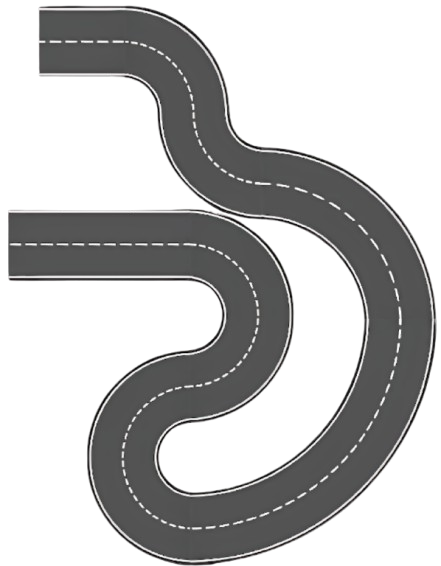
\includegraphics[width=0.5\textwidth]{/home/rgld_/01-dev-projects/cpp-projects/Driving-Sim/LaTeX/figures/example_circuit_1} % TODO FIX PATH
    \caption{Exemple de circuit pouvant être générer grâce à la classe Circuit}
    \label{fig:example_circuit_1}
\end{figure}

\paragraph[Car]{La classe \textbf{Car}}
Cette classe encapsule la classe \texttt{Vehicle} (voir section \ref{sec:l'implementation-de-la-physique-/-modelisation-d'un-systeme-de-dynamique-de-vehicule}).
L'interraction entre les deux classes \texttt{Car} et \texttt{Vehicle} est présenté à la section\ref{subsubsec:interactions-entre-l-interface-graphique-et-la-partie-physique}.
Elle calcul la ligne de prédiction de la trajectoire du véhicule et gère l'affichage du véhicule.

Lors du développement de la ligne de prédiction de trajectoire, nous avons rencontré un problème.
Le calcul prend en paramètre un delta de temps qui correspond au temps entre la dernière image et l'image actuelle.
Ce delta de temps est très volatile et peut varier du simple au double, ce qui cause des grosse différence de longueur de la ligne de prédiction et provoque une impression de scintillement.

Pour résoudre ce problème, nous avons décidé de récupérer le delta de temps médian sur les 1000 dernières images.

\begin{lstlisting}[style=CStyle, label={lst:code_dequeue_dt}]
std::deque<float> dtBuffer;
const size_t max_dt_buffer_size = 1000;
float updateAndGetMedian(const float dt) {
    dtBuffer.push_back(dt);
    if (dtBuffer.size() > max_dt_buffer_size) {
        dtBuffer.pop_front();
    }
    std::vector tmp(dtBuffer.begin(), dtBuffer.end());
    const auto mid = tmp.begin() + tmp.size() / 2;
    std::nth_element(tmp.begin(), mid, tmp.end());
    return *mid.base();
}
\end{lstlisting}

La complexité de la fonction \texttt{updateAndGetMedian(const float dt)} est en \( O(n) \).
Voici le détail de la complexité :
\begin{itemize}
    \item \texttt{push\_back(dt)} : \( O(1) \)\cite{cpp_reference_push_back} pour ajouter un élément à la fin de la deque.
    \item \texttt{pop\_front()} : \( O(1) \)\cite{cpp_reference_pop_front} pour retirer le premier élément de la deque.
    \item \texttt{std::vector tmp(dtBuffer.begin(), dtBuffer.end())} : \( O(n) \)\cite{cpp_reference_vector_copy} pour copier la deque dans un vecteur.
    \item \texttt{std::nth\_element(tmp.begin(), mid, tmp.end())} : \( O(n) \)\cite{cpp_reference_std_nth_element} pour trier le vecteur jusqu'à l'élément médian.
\end{itemize}

On a utilisé la fonction \texttt{std::nth\_element()} car elle permet de ne pas trier l'ensemble du vecteur tout en plaçant l'élément médian à la bonne position dans le \texttt{std::vector}.
Au départ, nous avions utilisé la fonction \texttt{std::sort()}, qui trie un vecteur complet, mais sa complexité aurait été en \( O(n \log n) \)\cite{cpp_reference_std_sort}, ce qui est moins optimal étant donné que la ligne de prédiction est recalculée à chaque image.

\paragraph[FPSCounter \& DebugMode]{Les Classes FPSCounter et DebugMode}
Ces deux classes sont dédiées à l'affichage d'informations de débogage et de performance.

La classe FPSCounter affiche le nombre de frames par seconde dans la HUD View, permettant ainsi de surveiller la fluidité de l'application.
Elle nous permet, tout au long du développement de remarquer si une fonctionnalité que l'on vient d'implémenter est trop gourmande en ressource et de l'optimiser en conséquence.
Pour calculer le nombre d'images par seconde, on compte le nombre d'images générer en une seconde.

La classe contient, parmi ses attributs, un compteur d'image \texttt{frameCount} et un accumulateur de temps \texttt{timeAccumulator}.
\begin{lstlisting}[style=CStyle, label={lst:code_fpscounter}]
void FPSCounter::update(const float dt) {
    timeAccumulator += dt;
    frameCount++;
    if (timeAccumulator >= 1.f) {
        currentFPS = frameCount;
        frameCount = 0;
        timeAccumulator = 0.f;
        text.setString("FPS: " + std::to_string(currentFPS));
    }
}
\end{lstlisting}
Le paramètre \texttt{dt} est le delta de temps entre la dernière image et l'image actuelle.


\subsubsection{Les ressources}\label{subsubsec:gestion-des-ressources}
\paragraph{Type de ressources}
Dans le projet, nous avons principalement deux types de ressources :
\begin{itemize}
    \item Les \textbf{Textures} : Utilisées pour le rendu graphique des segments de route et du véhicule.
    \item Les \textbf{Polices de caractères} : Utilisées pour le rendu du texte dans l'interface graphique.
\end{itemize}

\paragraph{Les textures}
Au sein de la librairie SFML, une image est représentée avec une classe \texttt{sf::Texture} qui contient la représentation en mémoire des pixels de l'image~\cite{sfml_sf_texture}.
Chaque texture (ou image) correspond à une entrée dans une enum \texttt{ResourceType::Value} qui permet de les identifier de manière unique, cela conserne les segments de route ainsi que l'image de la voiture.
Cette enum est définie dans le fichier \texttt{resource\_type.h} et contient les valeurs suivantes :
\begin{itemize}
    \item \texttt{SEGMENT\_SMALL\_STRAIGHT} : Une petite ligne droite.
    \item \texttt{SEGMENT\_LONG\_STRAIGHT} : Une grande ligne droite.
    \item \texttt{SEGMENT\_SMALL\_TURN} : Un virage moyen.
    \item \texttt{SEGMENT\_MEDIUM\_TURN} : Un virage moyen.
    \item \texttt{SEGMENT\_LARGE\_TURN} : Un virage large.
    \item \texttt{SEGMENT\_S\_TURN} : Un virage en S (plus communément appllé une chicane)
    \item \texttt{SEGMENT\_U\_TURN} : Un virage en U\@.
    \item \texttt{CAR} : La texture de la voiture.

\paragraph{La police d'écriture}
La police d'écriture utilisée dans le projet est la \textit{DejaVu Sans Mono}.
Pour plus de portabilité de notre code, nous avons décidé de l'inclure dans le projet.

Nous avons généré un fichier C++ contenant les données binaires de la police \textit{DejaVu Sans Mono} en utilisant la commande suivante :
\begin{lstlisting}[style=BashStyle,label={lst:generation_dejavusansmonottf_h}]
xxd -i DejaVuSansMono.ttf > dejavu_sans_mono_ttf.cpp
\end{lstlisting}
Cette commande convertit le fichier binaire de la police d'écriture en un tableau de bytes C++ que nous pouvons inclure directement dans notre projet.
Le fichier généré ressemble à ceci :
\begin{lstlisting}[style=CStyle,label={lst:example_generated_from_xxd_i}]
#include "dejavu_sans_mono_ttf.h"

unsigned char dejavu_sans_mono_ttf[] = {
  // Données binaires de la police d'écriture
};

unsigned int dejavu_sans_mono_ttf_len = 343140;
\end{lstlisting}
Cette solution, trouvée sur Stack Overflow\cite{stackoverflow_embed_font}, nous permet d'intégrer la police directement dans le binaire de l'application, assurant ainsi une portabilité maximale.

\paragraph{Gestionnaire de ressources}
Nous avons fait le choix de séparer la gestion de ces deux types de ressources en deux classes différente étant donné leurs utilisations différentes.
La classe \texttt{TextureManager} gère le chargement des images dans la mémoire de l'application.
Lorsque l'on a besoin d'utiliser une \texttt{sf::Texture}, on fait appel à la méthode \texttt{TextureManager::getTexture()} qui prends en paramètre un \texttt{ResourceType::Value} et renvoie un pointeur vers la texture correspondante.
Deux cas sont possibles :
\begin{itemize}
    \item La texture n'a jamais été demandé depuis le début de l'execution, elle est donc chargée depuis le disque dur et stockée dans une \texttt{std::unordered\_map<ResourceType::Value, sf::Texture>}.
    \item La texture a déjà été chargée, une référence vers la \texttt{sf::Texture} correspondante est récupérée puis renvoyée.
    Ici, on utilise une référence et non une copie, car aucun traitement n'est fait directement sur l'objet en mémoire.
\end{itemize}
Ce système permet de ne charger qu'une seule fois une texture et de la réutiliser à chaque fois qu'elle est demandée ce qui limite grandement l'utilisation de la mémoire.

Pour ce qui est des polices de caractères, la classe \texttt{FontManager} fonctionne de manière similaire, mais nous n'utilisons qu'une seule police de caractères pour l'ensemble de l'application.
Lors de la création de l'objet, la police est chargée depuis le disque dur et stockée dans un pointeur (\texttt{std::unique\_ptr<sf::Font>}) dans un attribut de la classe.


\paragraph{Connexion des segments de routes}
En interne la texture d'un segment de route est représenté par une structure \texttt{RoadTexture} défini comme suit :

\begin{lstlisting}[style=CStyle,label={lst:struct_roadtexture}]
struct RoadTexture {
    const sf::Texture *texture = nullptr;
    sf::Sprite sprite;
    sf::Vector2f point1;
    sf::Vector2f point2;
};
\end{lstlisting}

Elle contient 4 éléments :
\begin{itemize}
    \item \texttt{texture} : Un pointeur vers la texture de la route chargée par le \texttt{TextureManager}.
    \item \texttt{sprite} : Le sprite associé à la texture, utilisé pour le rendu. % TODO sprite => glossaire.
    \item \texttt{point1} et \texttt{point2} : Deux positions relatives à la texture représentant les points de connexion entre deux segments de route.
\end{itemize}

Lorsque l'on rajoute un segment de route dans le circuit à l'aide de la fonction \texttt{Circuit::join()}, la position du nouveau sprite est déterminé automatiquement grâce au précédent segment de route.
Le \texttt{point1} du nouveau segment est collée au \texttt{point2} du précédent segment, ce qui donne une impression de continuité.

% TODO Si changé, modifier le paragraph Car.
\subsubsection{Interactions entre l'interface graphique et la partie physique}\label{subsubsec:interactions-entre-l-interface-graphique-et-la-partie-physique}
Bien que l'implémentation de l'interface graphique soit distincte de la simulation physique, les deux composantes interagissent étroitement :
\begin{itemize}
    \item La classe \texttt{Car} récupère en temps réel les données issues du modèle physique (position, vitesse, trajectoire prédictive) afin de mettre à jour le sprite et le tracé de la trajectoire.
    \item La Game View est dynamiquement recentrée sur le véhicule pour garantir sa visibilité, même lors de mouvements rapides.
    \item La synchronisation entre les calculs physiques et l'affichage permet une expérience fluide et cohérente pour l'utilisateur.
\end{itemize}

\subsection{Composants et fonctionnalités}\label{subsec:composants-et-fonctionnalites}

\subsubsection{Affichage du véhicule et gestion de la vue}\label{subsubsec:affichage-du-vehicule-et-gestion-de-la-vue}

\paragraph{Rendu du sprite du véhicule}
Le véhicule est représenté par un sprite chargé via SFML. La classe \texttt{Car} initialise ce sprite en lui attribuant une texture provenant du gestionnaire de ressources, en définissant un point d'origine pour permettre une rotation naturelle et en appliquant un facteur de mise à l'échelle adapté à la taille de la fenêtre.
La position et l'orientation du sprite sont mises à jour à chaque cycle de la simulation afin de refléter l'état physique calculé.

\paragraph{Suivi du véhicule}
Pour que le véhicule reste toujours visible, la Game View est conçue pour suivre dynamiquement sa position.
Une méthode dédiée vérifie si le véhicule s'approche des limites de l'écran et demande à la classe \texttt{Game} de recentrer la vue.
Ce suivi adaptatif assure une expérience de simulation fluide, même en cas de changements brusques de direction ou de vitesse.

\subsubsection{Visualisation des informations dynamiques}\label{subsubsec:visualisation-des-informations-dynamiques}

\paragraph{Mode de Debug}
Le mode Debug offre une visualisation en temps réel de diverses informations physiques (vitesse, forces, angles, etc.). Activable par un raccourci clavier (F3), il affiche ces données sous forme de texte avec des arrière-plans colorés pour améliorer la lisibilité.
Cette fonctionnalité est particulièrement utile pour le débogage et l'analyse du comportement du véhicule.

\paragraph{Compteur de FPS}
Le compteur de FPS, géré par la classe \texttt{FPSCounter}, affiche le nombre de frames par seconde dans la HUD View.
Ce suivi de performance permet de vérifier en continu la fluidité de la simulation et d'identifier d'éventuels problèmes de performance, facilitant ainsi l'optimisation du code.

\subsubsection{Affichage de la trajectoire et prédictions}\label{subsubsec:affichage-de-la-trajectoire-et-predictions}

\paragraph{Calcul de la trajectoire prédictive}
Pour anticiper le comportement du véhicule, une trajectoire prédictive est calculée en itérant la dynamique sur plusieurs pas de temps.
Les positions successives sont stockées dans un tableau et affichées à l'écran sous forme de ligne continue, offrant ainsi à l'utilisateur un aperçu de l'évolution future du véhicule en fonction de ses actions actuelles.

\paragraph{Tracé en temps réel via les données issues de la simulation}
Le tracé de la trajectoire s'effectue en temps réel grâce à un objet \texttt{sf::VertexArray}.
À chaque mise à jour, les données prédictives sont utilisées pour reconstruire dynamiquement le chemin à afficher sur la Game View.
Cette visualisation interactive aide l'utilisateur à comprendre l'impact des commandes de conduite sur la trajectoire du véhicule.

\subsubsection{Gestion des événements utilisateurs}\label{subsubsec:gestion-des-evenements-utilisateurs}
La gestion des interactions se fait principalement via la méthode \texttt{manageEvents()} de la classe \texttt{Game} :
\begin{itemize}
    \item \textbf{Clavier} : La touche F active/désactive le compteur de FPS, F3 bascule le mode Debug, F5 réinitialise la position du véhicule et ESC ferme l'application.
    \item \textbf{Souris} : Le défilement de la molette permet d'ajuster le niveau de zoom sur la Game View, offrant ainsi à l'utilisateur la possibilité de mieux suivre le véhicule ou d'obtenir une vue d'ensemble du circuit.
\end{itemize}
Ce système d'événements assure une interactivité réactive et une expérience utilisateur intuitive.

\subsection{Optimisation du rendu et de l'affichage}\label{subsec:optimisation-du-rendu-et-de-l-affichage}
%TODO paragraph sur les view
Afin d'assurer une fluidité optimale du simulateur, plusieurs optimisations ont été mises en œuvre :
\begin{itemize}
    \item \textbf{Réduction des appels de dessin} : Les objets graphiques statiques (par exemple, le circuit ou les éléments du HUD) sont dessinés en une seule passe, tandis que les objets dynamiques (le véhicule, la trajectoire prédictive) sont mis à jour et redessinés à chaque frame.
    \item \textbf{Utilisation de Vertex Arrays} : Le tracé de la trajectoire est réalisé à l'aide d'un \texttt{sf::VertexArray}, ce qui permet de dessiner une série de points connectés en un seul appel de rendu.
    \item \textbf{Gestion efficace de la vue} : La Game View est ajustée dynamiquement en se recentrant sur le véhicule, minimisant ainsi les recalculs inutiles et garantissant que seul le contenu pertinent est redessiné.
\end{itemize}

\subsection{Perspectives d'amélioration et évolutions futures}\label{subsec:perspectives-d-evolution}
Bien que l'interface graphique actuelle réponde aux besoins du projet, plusieurs axes d'amélioration ont été identifiés pour de futures itérations :
\begin{itemize}
    \item \textbf{Effets visuels avancés} : L'ajout d'animations, d'effets de particules ou de transitions fluides pourrait enrichir l'expérience utilisateur.
    \item \textbf{Interface utilisateur interactive} : La mise en place de menus interactifs, d'options de configuration en temps réel ou d'indicateurs graphiques plus sophistiqués permettrait de personnaliser davantage la simulation.
    \item \textbf{Optimisation multi-threading} : La séparation des calculs physiques et du rendu graphique sur des threads distincts pourrait améliorer la réactivité et la fluidité de la simulation sur des systèmes multi-cœurs.
    \item \textbf{Extensions de la HUD View} : Intégrer davantage d'informations (comme des graphiques temps réel ou des indicateurs de performance détaillés) pourrait offrir un meilleur retour utilisateur.
\end{itemize}
